%
%-----------------------------------------------------------
%% Computer Music Journal LaTeX template
%%
%% September  2009
%% Author: Cornelia Kreutzer, University of Limerick



%---Document preamble
%
\documentclass[letterpaper, 12pt]{article}

\usepackage{cmjStyle} %use CMJ style
\usepackage{natbib} %natbib package, necessary for customized cmj BibTeX style
\bibpunct{(}{)}{;}{a}{}{, } %adapt style of references in text
\doublespacing
\raggedright % use this to remove spacing and hyphenation oddities
\setlength{\parskip}{2ex}
\parindent 24pt
\urlstyle{same} % make url tags have the same font
\setcounter{secnumdepth}{-1} % remove section numbering
\usepackage{epstopdf}
\usepackage{amsmath,amssymb,amsbsy,bm,upgreek,nicefrac}
\usepackage{todonotes,microtype}

%% ----------------------------------------------------------------------------------------------------------------------------------------
%% AUTHORS NOTE THE FOLLOWING:
%% You should not need any additional packages beyond those already listed above.
%% If you cannot resist the temptation to use further packages, add them under these lines,
%% including a brief description of each package and where you used it.
%% But consider that those packages will almost certainly be removed before sending your manuscript
%% to MIT Press for production.


% Use the Figures subfolder for image files
\graphicspath{{./Figures/}}

%% ----------------------------------------------------------------------------------------------------------------------------------------
%% CMJ page headers and footers
%%
%% For initial submission use \lhead{\small Anonymous}
%% On accepted for publication, use real author surnames for \lhead modeled on the following examples
%%              One author:     \lhead{\small Keislar}
%%              Two authors:    \lhead{\small Keislar and Castine}
%%              Three authors:  \lhead{\small Keislar, Castine, and Rundall}
%%              Four or more:   \lhead{\small Keislar et al.}
%%
\lhead{\small Anderson}

% Once accepted and the issue number is set, update the left-hand section of the footer to include volume and number
\lfoot{\small \emph{Computer Music Journal} Vol:No}

%% ----------------------------------------------------------------------------------------------------------------------------------------

%% The package endfloat moves all floats (figures, tables...) to the end of the manuscript, as required for the final version of a CMJ article.
%% AUTHORS: leave commented out when submitting to CMJ for editing
%% MS EDITOR: uncomment it and the callout commands prior when submitting for production to MIT Press.
% \usepackage{endfloat}
% \renewcommand{\figureplace}{%
%       \begin{center}
%               \textbf{<<TYPE: INSERT \figurename~\thepostfig\ ABOUT HERE.>>}
%       \end{center}}
% \renewcommand{\tableplace}{%
%       \begin{center}
%               \textbf{<<TYPE: INSERT \tablename~\theposttbl\ ABOUT HERE.>>}
%       \end{center}}

%% Display or Hide markups for production
%% (Hide markups for Just Accepted stage of Early Access, but provide MIT Press with a second copy with markups)
%\newcommand{\productionmarkup}[1]{}                                           % Markup hidden for JA
\newcommand{\productionmarkup}[1] {\textbf{<<#1>>}}             % Production markup displayed


%---Document----------
\begin{document}

{\cmjTitle Modeling performance nuance}
\vspace*{24pt}

{\cmjAuthor David P. Anderson}

\begin{cmjAuthorAddress}
Space Sciences Laboratory \\
University of California, Berkeley \\
davea@berkeley.edu \\
https://github.com/davidpanderson/numula/wiki
\end{cmjAuthorAddress}

\begin{abstract}

Music Nuance Model (MNM) is
a framework for describing performance nuance
(timing, articulation, dynamics, and pedaling) in notated music.
MNM can concisely express complex nuance,
such as that of human performances,
thus allowing musicians -- composers and performers --
to craft expressive renditions of musical works.
This capability has applications in composition, virtual performance,
and performance pedagogy.
I discuss the challenges in creating and refining
complex nuance specifications.

\end{abstract}

\section{Introduction}

This paper involves "performance nuance" in notated music;
by this I mean the differences between a rendition of a piece
and the score on which it's based.
Nuance has a central role in Western classical music:
works in the standard repertoire
are performed and recorded thousands of times,
and nuance is the primary difference among these renditions.

In the context of piano music, nuance has several components:

\textbf{Timing}: tempo, rubato, pauses, rolled chords,
and time-shifting of notes.

\textbf{Dynamics}: crescendos and diminuendos, accents, and chord voicing.

\textbf{Articulation}: legato, staccato, and portamento.

\textbf{Pedaling} (sustain, soft, and sostenuto),
including fractional pedaling.

Except for pedaling, these components apply to other
instruments (including voice) as well,
and to ensembles of instruments.
For many instruments, notes have additional properties such as attack,
and their timbre, pitch, and volume may vary during the note.
The work presented here does not address these factors
but might be extended to do so.

Many scores have nuance indications, such as
tempo markings, slurs, crescendo marks, fermatas, and pedal markings.
These indications do not completely describe the nuance in a human rendition
because
a) they're imprecise:
for example, a fermata sign doesn't specify the durations of the sound
and the following silence;
b) they're ambiguous:
the meaning of marks such as slurs, wedges, and staccato dots
has changed over time and varies between composers \citep{Bilson2005};
and c) they're incomplete:
they describe the broad strokes of the composer's intention,
but not the details of a rendition.
Indeed, Western music notation cannot express basic aspects of nuance,
such as the different volumes of notes in a chord.

In a typical human performance,
nuance is guided by additional factors:
the performer's expressive intent,
stylistic conventions as understood by the performer,
and the performer's technique and physical limitations.

Music Nuance Model (MNM) is a framework for describing performance nuance.
It defines a set of \textit{transformations} that
can be combined to describe complex nuance precisely and concisely.
MNM has several important properties:
\begin{enumerate}
\item
MNM can express nuance gestures that are continuous
(crescendos and accelerandos)
and/or discrete (accents and pauses).
It uses a powerful mechanism,
\textit{piecewise functions of time} (PFTs),
to describe time-varying quantities.
\item
MNM can express nuance gestures ranging from
short (pauses in the 10 millisecond range)
to long (say, an accelerando over 32 measures).
\item
MNM provides a general way of selecting sets of notes.
Notes can have textual tags,
and attributes such as chordal or metric position.
A note set is defined by a \textit{note selector},
a Boolean-valued function of these tags and attributes.
\item
MNM allows nuance to be factored into multiple layers.
Each layer, or \textit{transformation},
includes an operation type (e.g., tempo control), a PFT, and a note selector.
\end{enumerate}

As a way of shaping music,
MNM is intended to bridge the gap between score editors and DAWs.
It allows fine-grained control over each note,
using high-level constructs familiar to musicians,
expressed in the score time system.

The "reference implementation" of MNM is a Python library called Numula,
so I describe MNM in terms of Python data structures and functions.
MNM could be implemented using other languages or data representations.
It could be integrated into score editors, music programming languages,
or other music software systems.

MNM is designed to support systems in which a human musician
(not an AI or algorithm)
develops a nuance description for a work,
using an editing interface of some sort.
I call this \textit{nuance specification}.
It can be used, for example,
to create a virtual performance of a work,
or to communicate examples of nuance from teacher to student.

The remainder of this paper describes MNM and presents examples in which
it was used to create virtual performances of piano works in a range of styles.
I then discuss related and future work, and offer conclusions.

\section{The MNM model}

In the MNM model, a \textit{configuration}
represents a musical work, for a single instrument or an ensemble.
It is a collection of timed items such as notes, measures, and pedal usages.
MNM describes these as abstract classes:
\texttt{Configuration}, \texttt{Note}, \texttt{Measure}, and \texttt{PedalUsage}.
In Numula, these are Python classes.
The items in a configuration have associated start times and durations.
MNM uses two notions of time:

\textit{Score time} is time as notated (metrically) in a score,
represented as floating-point numbers.
The scale is arbitrary;
our convention is that the unit is a 4-beat measure,
so the duration of a quarter note is 1/4, or 0.25.
Score time is fixed,
and nuance adjustments are expressed in terms of score time.

\textit{Adjusted time} is a transformed version of score time.
A nuance adjustment can modify the
adjusted times of events (but not their score times).
After an MNM description has been applied to a configuration,
the final adjusted time is real time, measured in seconds.
Events with the same score time can have different adjusted times,
and score-time order can differ from adjusted-time order.

For clarity, I notate score time as $ s $ and adjusted time as $ t $.

MNM starts with an initial configuration $ C_0 $.
This might come from a score editor,
a MusicXML or MIDI file, or a Music21 object hierarchy;
or it could be generated programmatically.
Typically $ C_0 $ has no nuance:
adjusted times equal score times,
and notes have a default volume.

Applying a MNM nuance description to a configuration has two stages;
see Figure 1.
First, tags and attributes (see the following section)
are added to items in $ C_0 $,
producing a configuration $ C_1 $.
Next, a sequence of \textit{transformations} are applied.
Each transformation modifies a configuration:
for example, changing the volumes
or adjusted times of notes, or adding pedal usages.
This process produces configurations $ C_2, ..., C_n $.
The fully nuanced result is $ C_n $.
Its data (the volumes and adjusted times of its notes and pedal usages)
can be used to create an audio rendition using a synthesizer
or computer-controlled physical instrument.

\begin{figure}
    \begin{center}
    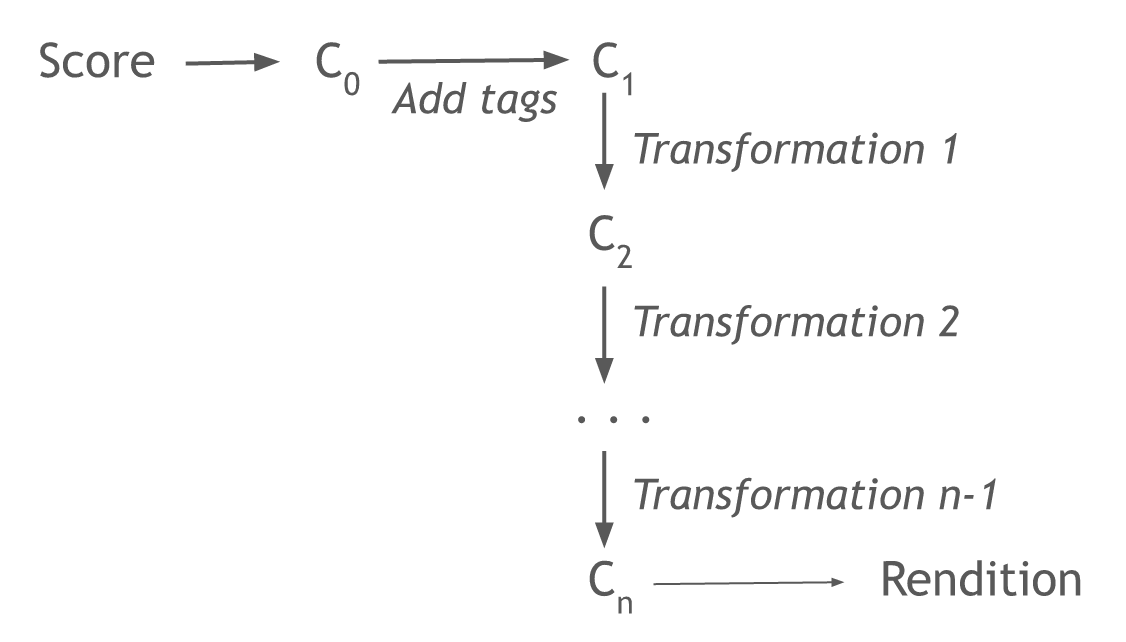
\includegraphics[width=120mm]{config2.png}
    \caption{MNM starts with an initial configuration $ C_0 $.
    Tags are added, resulting in $ C_1 $.
    Then transformations are applied in sequence, producing a nuanced result $ C_n $.}
    \label{fig:fig1}
    \end{center}
\end{figure}

Conceptually, each configuration $ C_i $ has its own adjusted time
system $ t_i $.
A timing adjustment maps $ t_i $ to $ t_{i+1},$
modifying the adjusted-time starts and durations of items.
The details are handled by Numula, and are not visible to the user.

\subsection{Attributes and tags}

A \texttt{Note} \texttt{N} has various \textit{attributes}.
For example, \texttt{N.tags} is a set of textual \textit{tags}.
Note attributes and tags are used to specify
the set of notes to which a transformation is to be applied.
This is done using \textit{note selector} functions, described below.

Note attributes and tags have various sources.
Some are derived from the score:
the start time and duration in score time (\texttt{N.s\_start} and \texttt{N.s\_dur}),
and the pitch \texttt{N.pitch} (represented, for example, as a MIDI pitch number).
If a score has information such as
slurs, accent marks, dynamic markings, and note stem directions,
these could be used to automatically assign attributes.
For ensemble works, a tag would indicate which instrument plays the note.

MNM assigns other attributes of a \texttt{Note} \texttt{N} based on its context in the score.
\texttt{N.nchord} is the number of notes
with the same start time as N, and \texttt{N.nchord\_pos}
is N's pitch order in this set (0 = lowest, 1 = 2nd lowest, etc.).
Tags "\texttt{top}" or "\texttt{bottom}" are added if N
has the highest or lowest pitch of notes starting at the same time.
If a note N lies within a measure M, N has two additional attributes:
\texttt{N.measure} is a reference to M,
and \texttt{N.measure\_offset} is N's score-time offset from the start of M.

Finally, the user can explicitly assign attributes and tags.
For example,
tags could indicate notes in the left and right hands
of a piano piece.
In a fugue, tags could indicate that a note is part of the fugue theme,
or of a particular instance of the theme.
Tags could indicate the harmonic function of notes;
e.g., a note in a dominant chord in a cadence,
or the 7th in a major seventh chord.
Attribute and tags could used to identify hierarchical
structural components of a work.
For example, one could tag notes in the development section of a Sonata.

Like notes, measures can have tags.
By convention, these include a string describing the measure's
duration and metric structure.
For example, the tag "\texttt{2+2+3/8}" might indicate a 7/8 measure
grouped as 2+2+3 eighths.

MNM does not specify or restrict how attributes and tags are assigned.
It can be done manually by a human nuance creator,
or automatically by the software system in which MNM is embedded.

\subsection{Note selectors}

A \textit{note selector} is a Boolean-valued function of a \texttt{Note}.
A note selector $ F $ identifies a set of notes within a \texttt{Configuration},
namely the notes $ N $ for which $ F(N) $ is True.
I use Python syntax for note selectors.
For example, the function

\begin{small}\begin{singlespace}\vspace{-18px}\begin{verbatim}
    lambda n: 'rh' in n.tags and n.s_dur == 1/2
\end{verbatim}\end{singlespace}\end{small}\vspace{-18px}\noindent
selects all half notes in the right hand, and
\begin{small}\begin{singlespace}\vspace{-18px}\begin{verbatim}
    lambda n: '3/4' in n.measure.tags and n.measure_offset == 2/4
\end{verbatim}\end{singlespace}\end{small}\vspace{-18px}\noindent
selects notes on the 3rd beat of 3/4 measures.
One can select notes based on any combination of note attributes:
score time, pitch, and so on.

In Python, the type of note selectors is:
\begin{small}\begin{singlespace}\vspace{-18px}\begin{verbatim}
    type NoteSelector = Callable[[\texttt{Note}], bool] | None
\end{verbatim}\end{singlespace}\end{small}\vspace{-18px}\noindent

\subsection{Piecewise functions of (score) time}

Nuance gestures typically involve values
(such as tempo and volume) that vary with time.
In MNM, these variations are described as functions of score time.
They are specified as a sequence of \textit{primitives},
each of which describes a function defined
either on a time interval or at a single time.
A function defined in this way is called a \textit{piecewise function of time}
(PFT).

In the reference implementation of MNM,
PFT primitives are objects with types derived from a base class \texttt{PFTPrimitive}.
There are two kinds of PFT primitives:

\textit{Interval primitives}
describe a function over a time interval $ [0, ds] $ where $ ds > 0 $.
Examples discussed below are
\texttt{Linear} (a linear function) and
\texttt{ShiftedExp} (a shifted exponential function).
Primitives could be defined for other types of functions
(polynomial, trigonometric, spline, etc.).

\textit{Momentary primitives} represent a value at a single moment.
Examples include
\texttt{Accent} (a volume accent),
\texttt{Pause} (a pause in timing), and
\texttt{Shift} (a shift in timing).

A PFT is a list of primitives:
\begin{small}\begin{singlespace}\vspace{-18px}\begin{verbatim}
    type PFT = list[PFTPrimitive]
\end{verbatim}\end{singlespace}\end{small}\vspace{-18px}\noindent

MNM uses PFT for various purposes, including tempo, articulation,
volume, time shifts, and pedaling.
When a PFT describes tempo, one needs
the definite integral of the function or of its reciprocal
(see the section "Timing" below).
Thus, primitives used in tempo PFTs must provide member functions
\begin{small}\begin{singlespace}\vspace{-18px}\begin{verbatim}
    integral(s: float): float               # integral of F from 0 to s
    integral_reciprocal(s: float): float    # integral of 1/F from 0 to s
\end{verbatim}\end{singlespace}\end{small}\vspace{-18px}\noindent

When a PFT is used for purposes other than tempo,
one needs the function value.
If there is a discontinuity in the PFT
(i.e. the ending value of a primitive differs
from the starting value of the next primitive),
one must specify which of these values is used.
Primitives used for these purposes must provide member functions

\begin{small}\begin{singlespace}\vspace{-18px}\begin{verbatim}
    value(s: float): float              # value at time s
    closed_start(): bool                # closure at time 0
    closed_end(): bool                  # closure at time ds
\end{verbatim}\end{singlespace}\end{small}\vspace{-18px}\noindent

For example, a volume control function might be defined by the PFT:
\begin{small}\begin{singlespace}\vspace{-18px}\begin{verbatim}
   [ Linear(25, 15, 2/1, closed_start = True),
     Linear(15, 20, 1/1, closed_end = True),
     Linear(10, 15, 2/1, closed_start = False) ]
\end{verbatim}\end{singlespace}\end{small}\vspace{-18px}\noindent

This defines a function that varies linearly
from 25 to 15 over two 4-beat measures,
from 15 to 20 over one measure,
then from 10 to 15 over two measures.
Its value at the start of the 4th measure is 20
because of the closure arguments;
see Figure 2.

\begin{figure}
    \begin{center}
    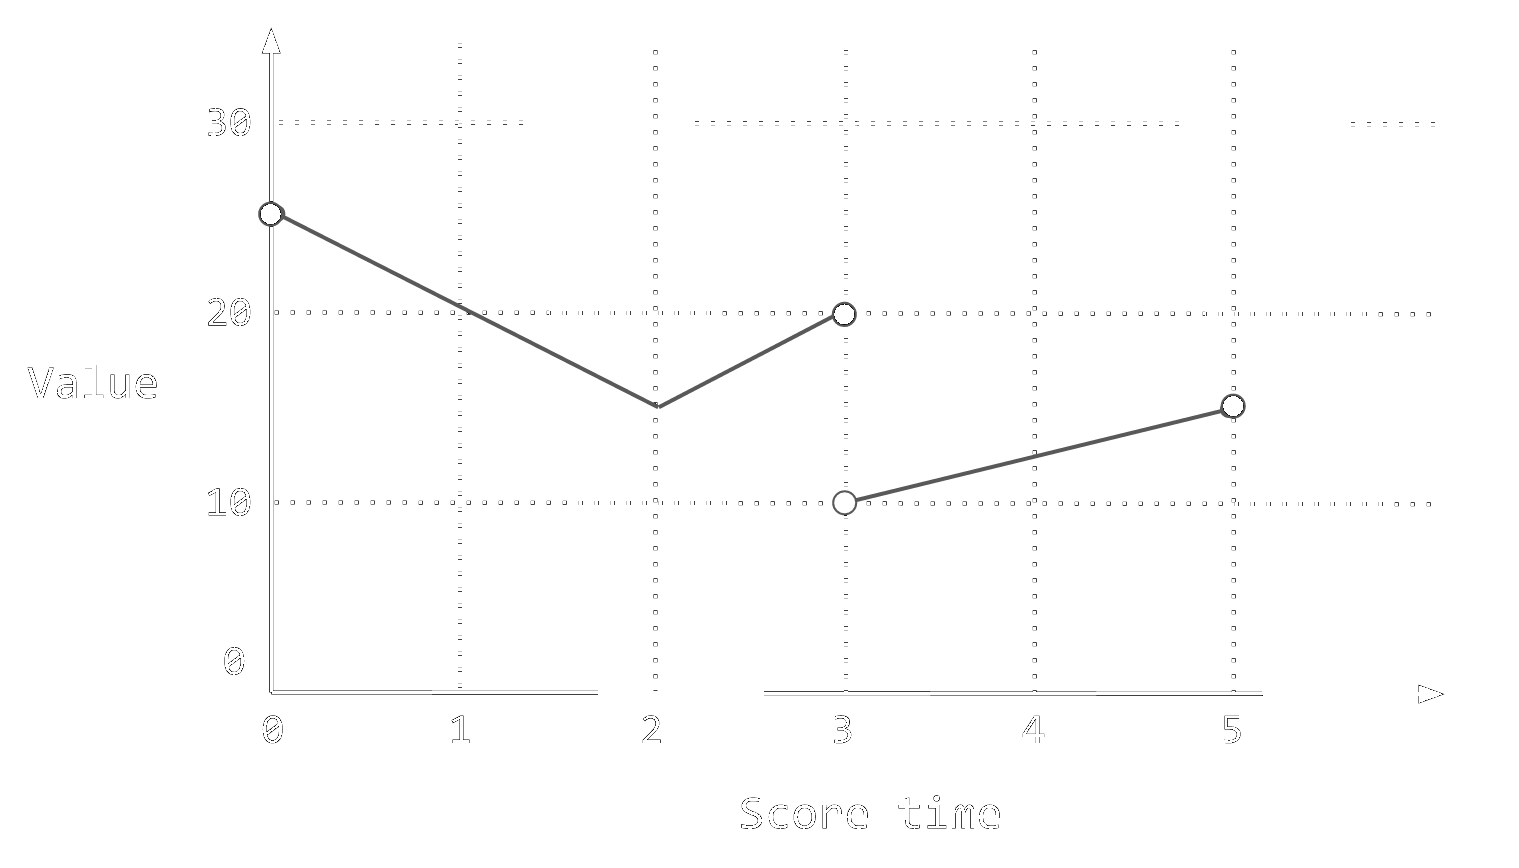
\includegraphics[width=120mm]{pft.png}
    \caption{A piecewise function of time is a concatenation of primitives.
Closure determines the function value at discontinuities.}
    \label{fig:fig2}
    \end{center}
\end{figure}

\subsubsection{Continuous PFT primitives}

The reference implementation of MNM has two continuous PFT primitives,
\texttt{Linear} and \texttt{ShiftedExp}.
Mathematical details are given in an Appendix.
The \texttt{Linear} primitive represents a linear function $ F $ with
$ F(0)=y_0 $
and
$ F(\Delta s)=y_1 $
.
The \texttt{ShiftedExp} primitive represents a family of
"shifted exponential" functions
$ F(t) $ that vary from $ y_0 $ to $ y_1 $ over
$ [0, \Delta s] $.
The primitive has a curvature parameter C.
If C is positive, F is concave up,
and its change is concentrated in the later part of the interval.
The larger C is, the more the change is shifted to the end.
Similarly, if C is negative,
change is concentrated in the earlier part of the interval.
If C is zero, F is linear.
Figure 3 shows examples.

\begin{figure}[]
    \begin{subfigure}{0.5\textwidth}
        \includegraphics[clip,width=\columnwidth]{exp2.png}
    \end{subfigure}
        \hfill
    \begin{subfigure}{0.5\textwidth}
        \includegraphics[clip,width=\columnwidth]{exp5.png}
    \end{subfigure}
        \hfill
    \begin{subfigure}{0.5\textwidth}
        \includegraphics[clip,width=\columnwidth]{exp-2.png}
    \end{subfigure}
        \hfill
    \begin{subfigure}{0.5\textwidth}
        \includegraphics[clip,width=\columnwidth]{exp-5.png}
    \end{subfigure}
    \caption{FIgure 3: Shifted-exponential primitives with different curvatures.}
    \label{fig:figMultipart}
\end{figure}

In developing nuance descriptions for a range of piano pieces
(see Examples below),
I found that these primitives were sufficient
to express the desired continuous variations in both tempo and volume.
It would be straightforward to add other primitives.

\subsubsection{Momentary PFT primitives}

MNM provides momentary primitives for several purposes.
\begin{small}\begin{singlespace}\vspace{-18px}\begin{verbatim}
    Accent(value: float)
\end{verbatim}\end{singlespace}\end{small}\vspace{-18px}\noindent
This represents a volume adjustment for notes that start
at a particular score time;
see the "Dynamics" section below.
The surrounding interval segments must be open at the corresponding end.

\begin{small}\begin{singlespace}\vspace{-18px}\begin{verbatim}
    Pause(duration: float, after: bool)
\end{verbatim}\end{singlespace}\end{small}\vspace{-18px}\noindent
This is used in tempo PFTs to represent a pause of the given duration,
in units of adjusted time.
If \texttt{after} is True, the pause occurs after the events
at the current score time;
otherwise it occurs before them.
There can be pauses both before and after a given time.

\begin{small}\begin{singlespace}\vspace{-18px}\begin{verbatim}
    Shift(value: float)
\end{verbatim}\end{singlespace}\end{small}\vspace{-18px}\noindent
This changes the adjusted times of events that start
at the current score time;
it does not affect later events.
It can be used for "agogic accents"
in which melody notes are emphasized by
shifting them slightly before or after accompaniment notes.

\subsection{Transformations}

An MNM specification includes a sequence of \textit{transformations}.
There is no limit on the number of transformations.
Each transformation acts on a \texttt{Configuration}, changing it in some way.
A transformation includes an "operator" indicating what it does.
I notate transformations as member functions of the \texttt{Configuration} class;
each function corresponds to an operator.
These functions are listed in the following sections.

The functions have various parameters.
Most include 1) a PFT describing a quantity
that varies as a function of score time,
2) a score time $ s_0 $ indicating when the transformation starts,
and 3) a note selector indicating which notes are affected.

Some transformations get values not from a PFT
but from a function that maps a \texttt{Note} to a number
(for example, a volume adjustment factor).
These arguments have the Python type
\begin{small}\begin{singlespace}\vspace{-18px}\begin{verbatim}
    type NoteToFloat = Callable[[Note], float]
\end{verbatim}\end{singlespace}\end{small}\vspace{-18px}\noindent

\section{Timing}

A note \texttt{N} has adjusted-time start and duration,
\texttt{N.t\_start} and \texttt{N.t\_dur}.
These are initially its score-time start and duration;
they can be changed by transformations.
MNM supports three kinds of timing transformations.

\textbf{Tempo control}: The adjusted times of note starts and ends
are changed according to a \textit{tempo function},
represented as a PFT.
The tempo function can include pauses.

\textbf{Time shifting}.
Note starts are shifted earlier or later in adjusted time.
Other notes are not changed
(unlike pauses, which delay all subsequent notes).

\textbf{Articulation control:} Note durations
are scaled or set to particular values,
expressing legato, portamento, or staccato.
This can be done in various ways,
including continuous variation of articulation using a PFT.

\subsection{Tempo control}

A tempo variation is described by a PFT
(a function defined over score time).
MNM provides three "modes" for this PFT:

\textbf{Slowness} (or inverse tempo):
The PFT value is the rate of change of adjusted time
with respect to score time.
If $ s_0 $ and $ s_1 $ are score times,
the PFT scales the interval from $ s_0 $ to $ s_1 $
by the average value of the PFT between those times.
Thus, larger means slower.

\textbf{Tempo}:
the PFT value is the rate of change of score time
with respect to adjusted time.
Intervals are scaled
based on the integral of the reciprocal of the PFT;
larger means faster.

\textbf{Pseudo-tempo}:
an approximation to Tempo mode for PFT primitive types for which
it's infeasible to compute the integral of the reciprocal.
Instead, the tempo parameters of the PFT primitives are inverted,
and the result is used as a slowness function.

In all cases, the PFT can also include momentary \texttt{Pause} primitives.
These are like Dirac delta functions, with zero width but positive integral.
The primitive's \texttt{before} parameter dictates whether
notes at the current score time are shifted.
The adjusted start times of later events are shifted by the pause duration.
In the case of a "before" pause at a time $ s $,
notes that start before $ s $ and end at $ s $ or later are elongated
to avoid introducing gaps in the sound.

The following transformation modifies the adjusted time of the selected notes,
starting at score time $ s_0 $,
according to the tempo function specified by the PFT,
acting in the given mode:
\begin{small}\begin{singlespace}\vspace{-18px}\begin{verbatim}
    Configuration.tempo_adjust_pft(
        pft: PFT,
        s0: float,
        selector: NoteSelector,
        normalize: bool,
        mode: int)           # one of the above modes
\end{verbatim}\end{singlespace}\end{small}\vspace{-18px}\noindent

The implementation of \texttt{tempo\_adjust\_pft()}, somewhat simplified,
is as follows (see Figure 4):

\begin{enumerate}
\item Make a list of all "events"
(starts and ends of the selected notes and of pedal applications)
ordered by score time.
Each event $ E $ has a score time $ E_s $ and
an initial adjusted time $ E_t $.
\item Scan this list, processing events 
whose score times lie within the domain of the PFT.
\item For each pair of consecutive events $ E1 $ and $ E2 $,
compute the average $ A $ of the PFT between $ E1_s $ and $ E2_s $
(that is,
the integral of the PFT over this interval divided by the interval size).
\item
Let
$ \Delta t $
be $ E2_t - E1_t $.
Set the new adjusted time of $ E2 $ to the (new) adjusted time of $ E1 $ plus
$ A \Delta t $.
\end{enumerate}

\begin{figure}
    \begin{center}
    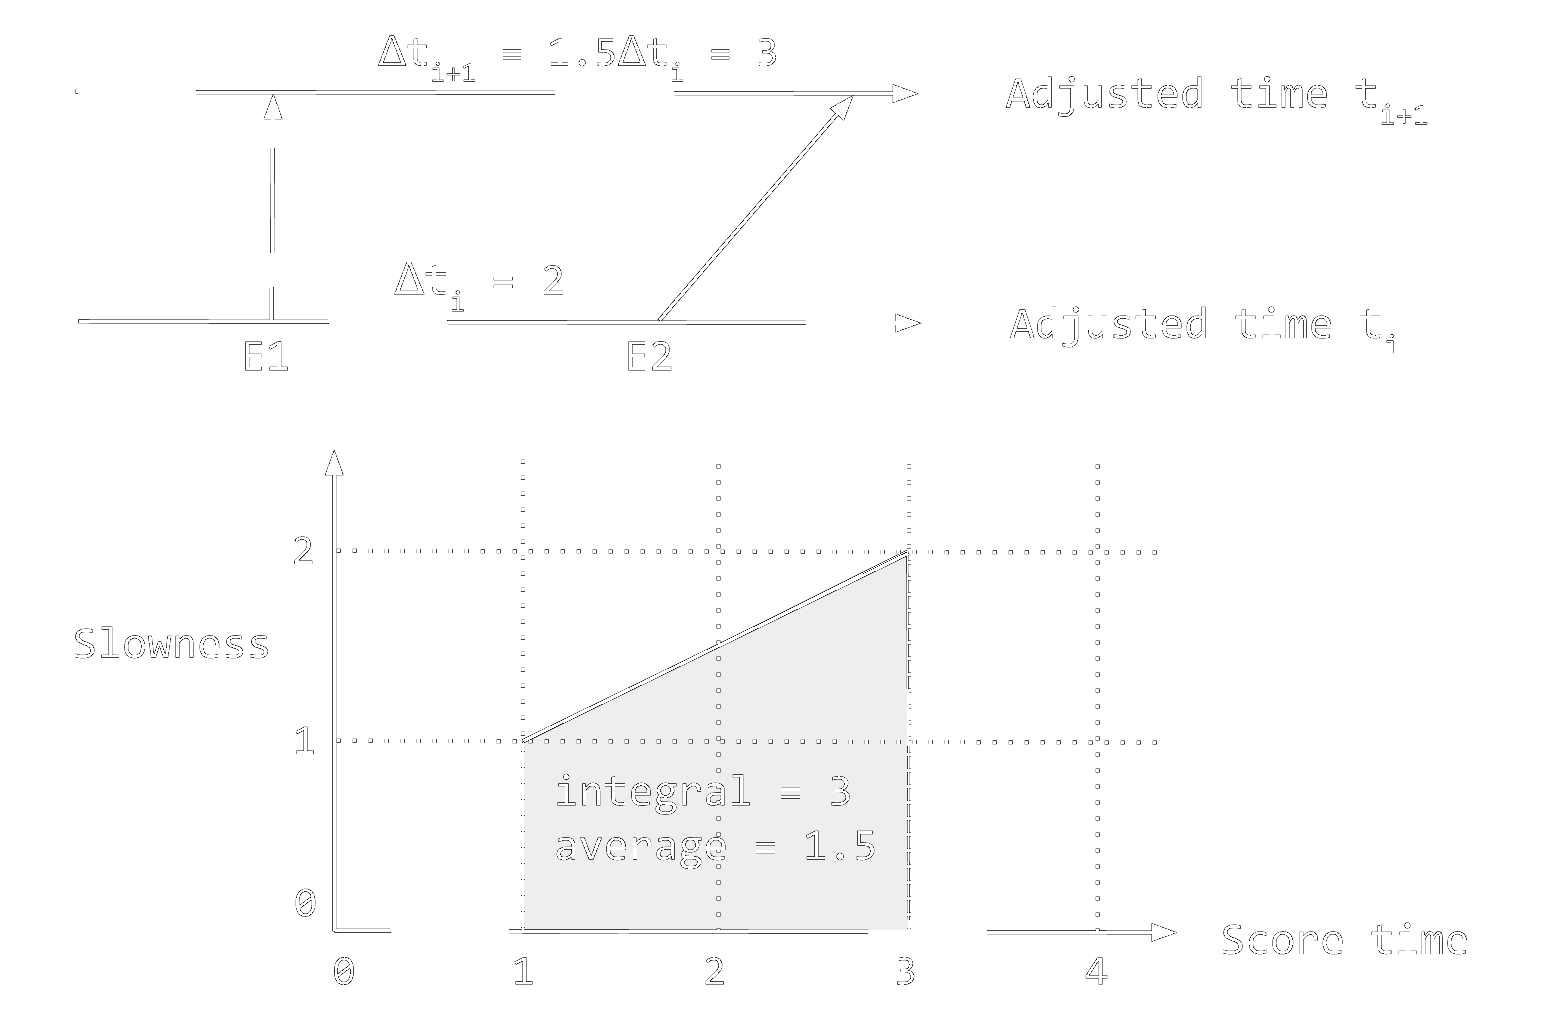
\includegraphics[width=120mm]{tempo2.png}
    \caption{Example of tempo adjustment.
Events $ E1 $ and $ E2 $ have score times 1 and 3,
and adjusted times determined by earlier transformations.
The interval in adjusted time between the events
is scaled by the average value of the slowness (inverse tempo) function
between their score times.}
    \label{fig:fig3}
    \end{center}
\end{figure}

It's important to understand that,
while a tempo adjustment maps one adjusted time system to another,
it does this using a tempo function defined
over score time (not adjusted time).
You can compose two or more tempo adjustments
simply by applying one after the other.
For example, one adjustment might slow down slightly over each measure,
while the second does an accelerando over 32 measures.
In this case, since the adjustments are multiplicative,
either order will produce this same result.
If the adjustments contain pauses, then order matters.

If \texttt{normalize} is set, the tempo adjustment is scaled
so that its average value is one;
in other words, the adjusted times of the start and end points remain fixed,
but events between them can move.
This can be used, for example, to apply rubato to
a particular voice over a given period,
and have the voice sync up with other voices at the end of that period.
For example, in a rendition Chopin's Nocturne No. 1
(see Figure 4),
I applied a tempo adjustment
consisting of an accelerando, a ritardando, and two small pauses
to the right-hand flourish.
This adjustment was normalized so that the left and right hands
sync up at the end of the figure.

\begin{figure}
    \begin{center}
    \includegraphics[width=120mm]{chopin.jpg}
    \caption{Example from Chopin's Nocturne No. 1.}
    \label{fig:fig4}
    \end{center}
\end{figure}

\subsection{Time shifts}

These transformations modify the adjusted start times of notes,
and change their durations to preserve the end times.

The following transformation,
for notes N that satisfy the selector and lie in the domain of the PFT,
adds \texttt{pft.value(N.s\_start - s0)} to \texttt{N.t\_start}:
\begin{small}\begin{singlespace}\vspace{-18px}\begin{verbatim}
    Configuration.time_shift_pft(
        pft: PFT,
        s0: float = 0,
        selector: NoteSelector)
\end{verbatim}\end{singlespace}\end{small}\vspace{-18px}\noindent
This can be used to give agogic accents to notes at particular times
or to shift notes by continuously varying amounts.

The following transformation "rolls" the chord at the given score time.
\begin{small}\begin{singlespace}\vspace{-18px}\begin{verbatim}
    Configuration.roll(
        s: float,
        offsets: list[float],
        is_up: bool = True,
        selector: NoteSelector)
\end{verbatim}\end{singlespace}\end{small}\vspace{-18px}\noindent
The \texttt{offsets} argument is a list of time offsets.
These offsets are added to the adjusted start times of notes
\texttt{N} for which \texttt{N.s\_start=s}.
If \texttt{is\_up} is True, the offsets are applied from the bottom pitch upwards;
otherwise they are applied from the top pitch downward.

The following transformation adds offsets
to the adjusted start times of notes satisfying the selector,
in order of increasing score time.
\begin{small}\begin{singlespace}\vspace{-18px}\begin{verbatim}
    Configuration.time_adjust_list(
        offsets: list[float],
        selector: NoteSelector)
\end{verbatim}\end{singlespace}\end{small}\vspace{-18px}\noindent
The \texttt{offsets} argument is a list of adjusted-time offsets.

The following transformation adds
adjusted-time offsets given by a function of the note:
\begin{small}\begin{singlespace}\vspace{-18px}\begin{verbatim}
    Configuration.time_adjust_func(
        f: NotetoFloat,
        selector: NoteSelector)
\end{verbatim}\end{singlespace}\end{small}\vspace{-18px}\noindent
For each note N satisfying the selector,
this adds \texttt{f(N)} to \texttt{N.t\_start}.
For example, the following adds Gaussian jitter to note start times:
\begin{small}\begin{singlespace}\vspace{-18px}\begin{verbatim}
    time_adjust_func(lambda n: 0.01*random.normal(), None)
\end{verbatim}\end{singlespace}\end{small}\vspace{-18px}\noindent
Adding such jitter can make renditions sound more human.

\subsection{Articulation}

Initially, the duration of a note is typically the time until
the next note in the same voice or part.
The following transformations control articulation by modifying note durations.
They involve an adjustment factor \texttt{A},
with three available modes:

\textbf{Absolute}: \texttt{N.t\_dur} is set to \texttt{A}.

\textbf{Multiplicative}: \texttt{N.t\_dur} is multiplied by \texttt{A}.

\textbf{Relative}: \texttt{N.t\_dur} is set so that the gap between \texttt{N}
and the next note is \texttt{A}.

The following transformation adjusts the adjusted durations of selected notes
based on a PFT;
it can be used to change articulation continuously.
\begin{small}\begin{singlespace}\vspace{-18px}\begin{verbatim}
    Configuration.dur_adjust_pft(
        pft: PFT,
        mode: int,          # one of the above modes
        t0: float,
        selector: NoteSelector)
\end{verbatim}\end{singlespace}\end{small}\vspace{-18px}\noindent

The following transformation adjusts durations
of selected notes \texttt{N} using the adjustment factor
given by a function \texttt{f(N)}.
\begin{small}\begin{singlespace}\vspace{-18px}\begin{verbatim}
    Configuration.dur_adjust_func(
        f: NotetoFloat,
        mode: int,
        selector: NoteSelector)
\end{verbatim}\end{singlespace}\end{small}\vspace{-18px}\noindent

\subsection{Layering timing transformations}

PFT-based tempo transformations without pauses commute,
so the order in which they're applied doesn't matter.
Other transformations generally don't commute.
The recommended order of transformations is
1) tempo transformations;
2) pause transformations;
3) shift transformations;
4) articulation transformations.

\section{Pedal control}

Grand pianos typically have three pedals:

\textbf{Sustain pedal}: when fully depressed,
the dampers are lifted so that
notes continue to sound after their key is released,
and all strings vibrate sympathetically.
If the pedal is gradually raised, the dampers are gradually lowered.
Pianists use this "half pedaling" (or more generally, fractional pedaling)
to create various effects.

\textbf{Sostenuto pedal}: like the sustain pedal,
but when it is depressed, only the dampers
of currently depressed keys remain lifted.
Half-pedaling works similarly to the sustain pedal.

\textbf{Soft pedal}: this shifts hammers horizontally so that they
contact only 2 of the 3 strings of treble notes,
reducing loudness and softening the timbre.
Fractional pedaling can also be used; its effects vary between pianos.

Pedaling, including fractional pedaling,
is critical to the sound of most performances,
but few composers notate it at all, much less completely and precisely.
Notation of fractional pedal is rare.
Most MIDI piano synthesizers implement all three pedal types.
Some, such as Pianoteq, also implement fractional pedaling.

\subsection{Control of standard pedals}

MNM provides a mechanism for specifying the use
of standard grand-piano pedals.
The level of a particular pedal can be specified as a PFT
with values in $ [0,1] $,
where 1 means the pedal is fully depressed and 0 means it's lifted.
For example,
\begin{small}\begin{singlespace}\vspace{-18px}\begin{verbatim}
    Linear(4/4, 1.0, 0.5)
\end{verbatim}\end{singlespace}\end{small}\vspace{-18px}\noindent
represents a gradual pedal change from fully depressed to half depressed
over 4 beats.
If MNM is being used to generate MIDI output, this produces
a sequence of continuous-controller commands
with values ranging from 127 to 64.

The following transformation applies a pedal of the given type,
with values described by a PFT, starting at score time $ s_0 $:
\begin{small}\begin{singlespace}\vspace{-18px}\begin{verbatim}
    Configuration.pedal_pft(
        pft: PFT,
        type: int,      # sustain, sostenuto, or soft
        s0: float)
\end{verbatim}\end{singlespace}\end{small}\vspace{-18px}\noindent

When a pedal change is simultaneous with note starts,
one needs to specify
whether the change occurs before or after the notes are played.
For sustain and sostenuto pedals,
one may also need to specify a momentary lifting of the pedal.
MNM handles both requirements using the closure attributes
of PFT primitives.
Suppose that P0 and P1 are consecutive primitives;
P0 ends and P1 begins at time t,
and one or more notes start at t.
The semantics of the PFT depend on the closure of P0 and P1 as follows
(\texttt{P1.y0} denotes the initial value of P1):

\begin{small}\begin{singlespace}\vspace{-18px}\begin{verbatim}
end of P0   start of P1     Semantics
-------------------------------------
open        open            lift pedal, play notes, pedal=P1.y0
open        closed          lift pedal, pedal=P1.y0, play notes
closed      open            play notes
closed      closed          play notes, pedal=P1.y0
\end{verbatim}\end{singlespace}\end{small}\vspace{-18px}\noindent

\subsection{Virtual sustain pedals}

It's sometimes musically useful to sustain only certain keys (pitches).
The sustain pedal can't do this: it affects all keys.
The sostenuto pedal affects a subset of keys, but its use is limited.
MNM provides a mechanism, \textit{virtual sustain pedal},
that's like a sustain pedal that affects only a specified set of notes.

A virtual sustain pedal usage
is specified by the same type of PFT as for standard pedals,
but the only allowed values are 0 (pedal off) or 1 (pedal on).
The following transformation applies a virtual sustain pedal:
\begin{small}\begin{singlespace}\vspace{-18px}\begin{verbatim}
    Configuration.virtual_sustain_pft(
        pft: PFT,
        s0: float,
        selector: NoteSelector)
\end{verbatim}\end{singlespace}\end{small}\vspace{-18px}\noindent
If a note N is selected, and the virtual pedal is on at its start time,
\texttt{N.s\_dur} is adjusted so that N is sustained at least until the
pedal is released.

One can use virtual sustain pedals, for example,
to sustain an accompaniment figure without affecting the melody.
In the Chopin example in Figure 4,
I used a virtual sustain pedal to sustain the chords in the left hand
without blurring the right-hand melody.
This would be impossible in a physical performance.

Compared to standard pedals,
virtual sustain pedals are more flexible
in terms of what notes are sustained.
Since they affect only note durations,
they lack two features of standard pedals: there is no fractional pedal,
and there is no sympathetic resonance of open strings.

\subsection{Pedal layering}

In an MNM nuance description,
pedal specifications must precede timing adjustments
so that pedal timing is correct.
Timing adjustments (including time shifts)
affect pedal usages as well as notes.
For virtual pedals, this happens automatically.
For standard pedals, if a note at time T is shifted backward in time,
pedals active at T are shifted backward by the same amount.

Uses of the standard pedals can't be layered;
that is, PFTs controlling a particular pedal can't overlap in time.
However, virtual sustain PFTs can overlap standard pedal PFTs.

\section{Dynamics}

In MNM, the volume of a note is represented by a floating-point number
in [0..1] (soft to loud).
This may be mapped linearly to a MIDI velocity [0..127];
the perceived loudness depends on the synthesis engine and other factors.
Notes initially have volume 0.5.

MNM provides three modes of volume adjustment.
In each case there is an adjustment factor A,
which may vary with time.

\texttt{VOL\_MULT}: the note volume is multiplied by A,
which typically is in [0..2].
This maps the default volume (0.5) to the full range [0..1].
These adjustments are commutative.

\texttt{VOL\_ADD}: A is added to the note volume.
A is typically around 0.1 or 0.2.
This is useful for bringing out melody notes when the overall volume is low.

\texttt{VOL\_SET}: the note volume is set to A/2.
A is in [0..2].
The division by 2 means that the scale is the same as for \texttt{VOL\_MULT}.

Multiple volume adjustments can result in levels outside [0..1],
in which case a warning is generated and the volume is truncated.

The following transformation adjusts the volume of selected notes
according to values specified by a PFT:

\begin{small}\begin{singlespace}\vspace{-18px}\begin{verbatim}
    Configuration.vol_adjust_pft(
        mode: int,          # one of the above modes
        pft: PFT,
        s0: float,
        selector: NoteSelector)
\end{verbatim}\end{singlespace}\end{small}\vspace{-18px}\noindent

If a note \texttt{N} is selected and is in the domain of the PFT,
its volume is adjusted by the factor given
by the value of the PFT at time \texttt{N.s\_start - s0}.
This can be used to shape the dynamics of a voice or of the piece as a whole.

Other transformations adjust note volumes without a PFT:
\begin{small}\begin{singlespace}\vspace{-18px}\begin{verbatim}
    Configuration.vol_adjust(
        mode: int,
        factor: float,
        selector: NoteSelector)
    Configuration.vol_adjust_func(
        mode: int,
        func: NoteToFloat,
        selector: NoteSelector)
\end{verbatim}\end{singlespace}\end{small}\vspace{-18px}\noindent
These adjust the volumes of the selected notes.
For \texttt{vol\_adjust\_func()}, the 2nd argument is a function
that maps a \texttt{Note} to an adjustment factor.
For example, in a piece with 4/4 measures,
the following transformations de-emphasize notes on weak beats:
\begin{small}\begin{singlespace}\vspace{-18px}\begin{verbatim}
    config.vol_adjust(VOL_MULT, 0.9, lambda n: n.measure_offset == 2/4)
    config.vol_adjust(VOL_MULT, 0.8, lambda n: n.measure_offset in [1/4, 3/4])
    config.vol_adjust(VOL_MULT, 0.7,
        lambda n: n.measure_offset not in [0, 1/4, 2/4, 3/4]
    )
\end{verbatim}\end{singlespace}\end{small}\vspace{-18px}\noindent

\subsection{Layering volume transformations}

Volume transformations can be layered.
Multiplicative transformations commute, so their order doesn't matter.
Other transformations generally do not commute.
A typical order:
transformations with mode \texttt{VOL\_MULT},
followed by transformations with mode \texttt{VOL\_ADD},
then transformations with mode \texttt{VOL\_SET}.

\section{The process of specifying nuance}

I designed MNM to enable a human musician (composer or performer)
to manually create a nuance description for a work.
I call this process \textit{nuance specification}.
It's analogous to practicing the work on a physical instrument.
You (the musician)
start by forming a mental model of how you want the piece to sound.
You create a rough draft of a nuance description.
Then you iteratively edit the description
to bring it closer to your mental model
(which may evolve in the process).

I created nuance specifications for piano pieces in several styles,
with the goal of achieving expressive and human-like virtual performances
(see "Examples" below).
This section
describes some principles and techniques that I found useful.

\subsection{Note tagging}

The first step in creating a draft specification
is to identify sets of notes that are to be treated specially,
and assign corresponding tags to those notes.
For example, you might tag notes as melody or accompaniment,
or as being in the left- or right-hand part.
Notes can have multiple tags, so these sets can overlap.

\subsection{Nuance structure}

The next step is to decide on a \textit{nuance structure}:
a sequence of transformation types, each with a particular purpose.
The goal is that when you want to change the sound in a particular way,
it's clear which layer is involved.
I typically use, for both timing and dynamics:
\begin{enumerate}
\item Layers of continuous transformation at multiple time scales:
typically a layer at the phrase level (1-8 measures or so)
and a layer at a shorter time scale (1 measure or less).
\item A layer of repeating discrete change
(for example, patterns of accents on the beats within a measure,
or pauses within a measure).
\item A layer of irregular discrete change
(for example, pauses at phrase ends
or agogic accents on particular melody notes).
\end{enumerate}

Layers can apply only to note subsets:
for example, the left- and right-hand parts,
an accompaniment, or a melody.

For pedal control, I typically use
a PFT for the standard sustain pedal,
and PFTs for virtual sustain pedals that affect only some voices,
typically accompaniment.

\subsection{Refining nuance specifications}

You create an initial "rough draft"
of tempo and volume changes based on score markings and
musical intuition.
This is followed by an iterative refinement process.
At the lowest level, this involves an editing cycle:
\begin{enumerate}
\item Listen to part of the rendition.
\item Identify a deviation from your mental model.
\item Locate and change the relevant part of the nuance description:
for example, a parameter of a PFT primitive.
\end{enumerate}

This cycle may repeat hundreds of times,
so it should ideally be streamlined.
I found that I continued to edit nuance
only as long as the reward exceeded the effort.

You also need a high-level editing strategy.
I found the following guidelines useful:
a) work on a short part of the piece (say, one measure or phrase);
b) work on one voice at a time
(it may be useful to hear other voices at the same time);
c) work on one nuance layer at a time
(it may be useful to enable other layers at the same time).
When you're done editing a section,
collect the transformations into a function (see below)
that you can reuse in similar sections later in the piece.

High- and low-level editing are intertwined.
While doing low-level editing,
you may decide to make high-level changes,
such as adding note tags or changing the nuance structure.

\section{Nuance description files and scripting}

It's natural to want the ability to store nuance data in a specialized file:
a \textit{nuance description file} (NDF).
Ideally, musicians should be able to share these by email,
upload them to archival sites,
manage versions on Github, and so on.
Software systems implementing MNM should be able to
export and import NDFs.

There are many possibilities for the content and format of NDFs.
With Numula, an NDF is a Python program.
Compared with other formats,
this has the advantage of being \textit{scriptable}: it can express:

\textbf{Iteration}:
defining a dynamic pattern once and applying it 16 times,
rather than repeating the definition 16 times.

\textbf{Parameterization}:
using variables instead of hard-coding values for PFT primitive parameters,
so that a single change can affect many places.

\textbf{Functions}:
generating PFTs or sets of transformations using functions,
possibly with parameters, loops, conditionals, recursion, and so on.

In my experience, these capabilities are essential for
describing complex nuance for long works.

At the other end of the spectrum,
an NDF could be a static (non-scriptable) data structure, encoded in JSON.
This would include two parts:
a) tagging information:
for each note (identified, perhaps, by score time and pitch)
a list of tags and attributes;
and b) a list of transformations, each with a PFT and a note selector
(a Boolean expression, e.g. in Python syntax).
This format would suffice for many purposes,
and its display in a graphical score editor would be straightforward.
It lacks scripting features,
but these could possibly be added in some form;
this is an area of future work.

\section{User interfaces for editing nuance descriptions}

There are many possible user interfaces for creating
and editing MNM nuance descriptions.
Desiderata for such interfaces include
a) access to all MNM features:
PFTs, transformations, note selectors, and so on;
b) support for nuance scripting;
and c) ease of use; in particular, an efficient editing cycle.
I propose four general approaches:
graphical, textual, performative, and conductive.

\textbf{Graphical}:
Nuance transformations might, for example,
be displayed as "tracks",
with their PFTs shown graphically as functions of time.
The mouse is used to drag and drop nuance primitives,
and to adjust their parameters.
This interface could be integrated with a graphical score editor
such as Musescore or Sibelius;
transformations would be displayed underneath the
corresponding part of the score.
The interface might also convey nuance by altering
the score's graphical components:
for example, note-head color or size could express dynamics,
and horizontal position could show adjusted time.

Making a graphical interface scriptable is a challenge.
The interface might allow copy-and-paste of units of nuance
such as dynamic-control shapes.
It would need to allow these copies to be linked,
so that a change in one is automatically propagated to the others.
Features like iteration and functions
would require either a scripting language,
as in systems like Max (Puckette 2002),
or a graphical programming language like Scratch (Resnick 2009).

\textbf{Textual}:
For example, MNM could be presented as an API in a programming language;
Numula uses Python for this purpose.
The user describes nuance by writing code.
The system might also allow programmatic description of scores.
Scriptability is inherent in this approach.
Alternatively, an existing system for textual score specification,
such as Lilypond (Nienhuys 2003),
might be extended both to include nuance and to be scriptable.

Ease of use is a challenge for textual systems.
First, if one uses the native programming language syntax
(data structure declarations and function calls),
the amount of typing can be prohibitive.
Numula addresses this by defining
textual "shorthand notations" for various purposes,
such as volume and tempo PFTs.
The second issue is the efficiency of the editing cycle.
If the user has to scroll through a text file,
locate and edit some text, and then rerun a program,
it adds up to perhaps a dozen input actions.
This is cumbersome; dealing with syntactic issues can cause
the user to lose musical focus.
Numula addresses this issue, in part,
using a feature in which parameter adjustment
and playback are done with single keystrokes (see below).



\textbf{Performative}:
the user inputs nuance gestures by performing parts of the score
on a computer-interfaced instrument or by singing.
For example, one plays a melody,
and the system captures the tempo and volume contours,
representing them as MNM transformations
that are then used in a textual or graphical editor.



\textbf{Conductive}:
the user inputs nuance gestures by "conducting" them in some way,
perhaps using a mouse, touch screen, or a baton-like input device.


Each of these approaches has strengths and weaknesses.
They potentially can be combined.
For example, a system might use a performative and conductive interface
to input large nuance gestures with coarse resolution,
then use a graphical or textual interface to refine the large gestures
and add smaller ones.

\section{Applications of nuance specification}



Nuance specification has several potential applications.


\textbf{Composition}:
As a composer writes a piece,
perhaps using a score editor such as MuseScore or Sibelius,
they develop a nuance description in parallel.
The audio rendering function of the score editor
uses this to produce nuanced renditions of the piece.
This facilitates the composition process
and allows the composer to convey their musical intentions
to prospective performers.




\textbf{Virtual performance}:
Musicians create nuanced renditions of existing pieces
using a computer rather than a physical instrument.
Compared to physical performance, this has several advantages:
performers are not limited by their physical capabilities,
they can return to working on a piece without having to relearn it,
and multiple performers can collaborate on a rendition.



\textbf{Performance pedagogy}:
A piano teacher's instruction to a student involves
a nuance specification that guides the student's practice.
Feedback might be given in various ways.
For example, as a student practices a piece, they see a
"virtual conductor" showing, on a screen,
a representation of the target nuance.
Or a "virtual coach" makes suggestions
(musical or technical) to the student based on
the differences between their playing and the nuance specification.



\textbf{Ensemble rehearsal and practice}:
When an ensemble (say, a piano duo) rehearses together,
they record their interpretive decisions as a nuance specification.
They then use this to guide their individual practice
(perhaps via a "virtual conductor" as described above).



\textbf{Musical collaborations}:
A dance troupe or musical theater group might
not be able to afford live musicians for rehearsals.
Instead, the group develops a specification of the nuance they want,
uses it to synthesize music for rehearsals,
and sends it to the musicians to help them prepare for performance.



\textbf{Automated accompaniment}:
a computer system might better track a human performer
given a description of the nuance
the performer is likely to use.



\textbf{Sharing and archival of nuance descriptions}:
Web sites like IMSLP (https://imslp.org)
and MuseScore (https://musescore.com) let people share scores.
Such sites could also host user-supplied nuance descriptions,
allowing people to share and discuss interpretations.

\section{Numula}

Numula is a Python library for creating nuanced music.
It consists of several modules; see Figure 6.
These modules can be used separately or in combination,
and they could be integrated into other systems.

\begin{figure}
    \begin{center}
    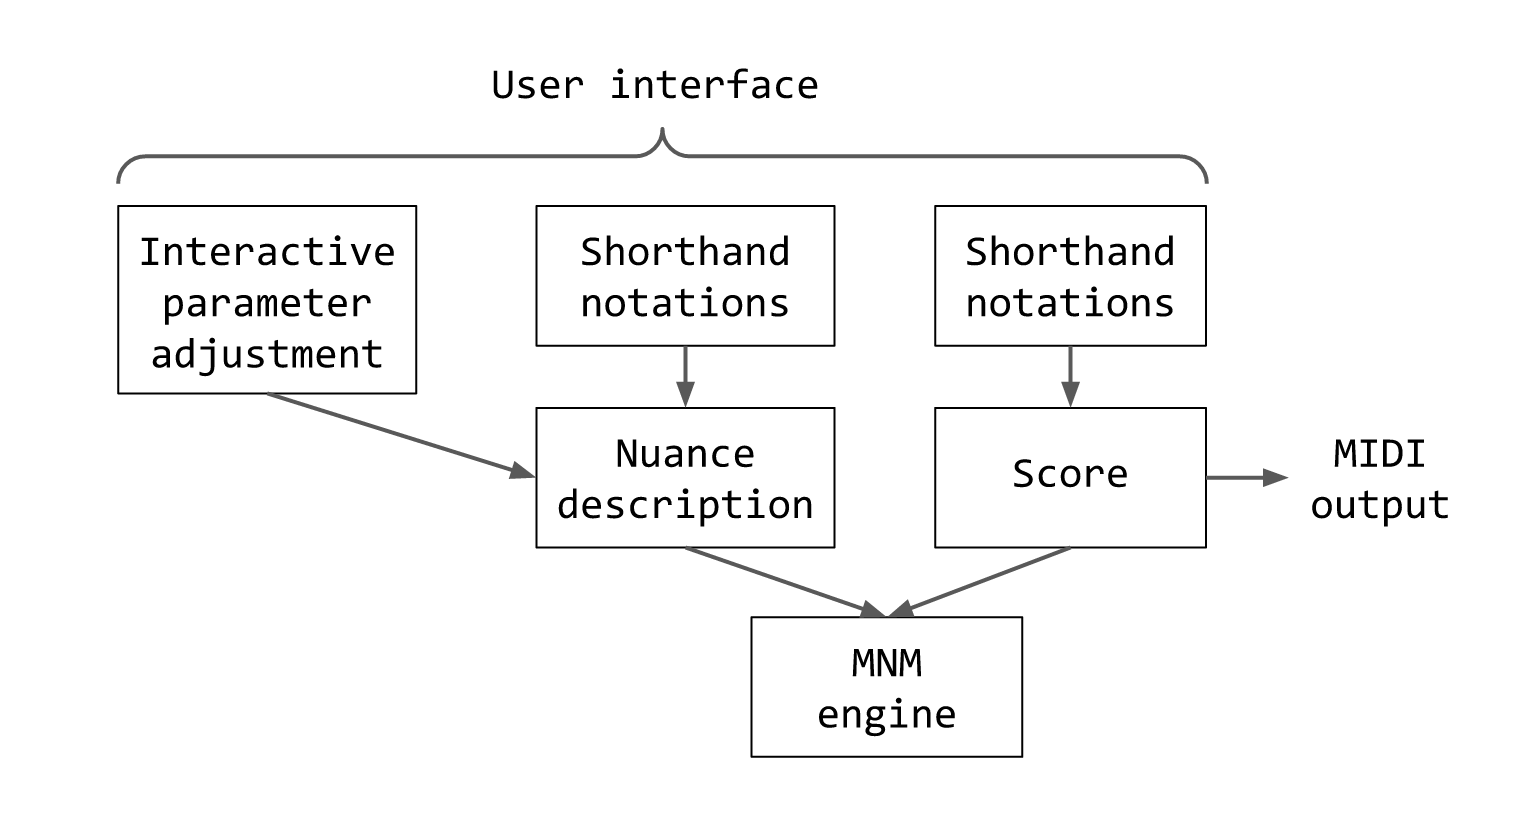
\includegraphics[width=120mm]{numula.png}
    \caption{The components of Numula.}
    \label{fig:fig5}
    \end{center}
\end{figure}

Numula defines the classes listed earlier in this paper:
\texttt{Configuration}, \texttt{Note}, PFT, etc.
The transformation functions described in earlier sections
are members of the \texttt{Configuration} class;
they form the "MNM engine".
A \texttt{Configuration}, after nuance transformations are applied,
can be output as a MIDI file.
For convenience, Numula can be configured to play MIDI output
using a Pianoteq server controlled by RPCs.

Numula can be used as a stand-alone system for creating nuanced music.
Alternatively, it can add nuance capabilities to other systems:
it can import a MIDI file as a \texttt{Configuration} object,
apply a nuance description to it,
and output the result as a MIDI file.

\subsection{Shorthand notations}

Numula provides textual \textit{shorthand notations}
for describing scores and various types of PFTs
(tempo, volume, pedal, and so on).
These notations require much less typing (and time) than
describing the scores and PFTs directly in Python.
They also reduce the need to write Python code,
making Numula more accessible to non-programmers.

Each type of shorthand notation has its own syntax.
For example,
\begin{small}\begin{singlespace}\vspace{-18px}\begin{verbatim}
    sh_vol('pp 2/4 mf 4/4 pp')
\end{verbatim}\end{singlespace}\end{small}\vspace{-18px}\noindent
returns a volume-control PFT representing a crescendo
from \textit{\textbf{pp}} to \textit{\textbf{mf}} over 2 beats,
then a diminuendo to \textit{\textbf{pp}} over 4 beats
(\texttt{pp} and \texttt{mf} are constants representing 0.45 and 1.11 respectively);
\begin{small}\begin{singlespace}\vspace{-18px}\begin{verbatim}
    sh_tempo('60 8/4 80 p.03 4/4 60')
\end{verbatim}\end{singlespace}\end{small}\vspace{-18px}\noindent
returns a PFT for a tempo that varies linearly from 60 to 80 BPM
over 8 beats,
a pause of 30 milliseconds after that point,
then linearly back to 60 BPM over 4 beats;
\begin{small}\begin{singlespace}\vspace{-18px}\begin{verbatim}
    sh_pedal('1/4 (1/4 0 1.) (1/4) 4/4')
\end{verbatim}\end{singlespace}\end{small}\vspace{-18px}\noindent
returns a PFT for a pedal that's off for 1 beat,
changes linearly from off to on over 1 beat,
is on for 1 beat, then off for 4 beats; and
\begin{small}\begin{singlespace}\vspace{-18px}\begin{verbatim}
    sh_score('1/4 c5 d e')
\end{verbatim}\end{singlespace}\end{small}\vspace{-18px}\noindent
returns a \texttt{Configuration} with 3 quarter notes starting at middle C.
Numula's shorthand notation for scores has numerous features
that enable compact representation of complex scores.

The shorthand notations have a common set of features
that increase their expressive power:

\textbf{Iteration}:
a string surrounded by \texttt{*N ... *} is repeated N times.
For example,
\begin{small}\begin{singlespace}\vspace{-18px}\begin{verbatim}
    sh_tempo('*4 60 8/4 80 p.03 4/4 60 *')
\end{verbatim}\end{singlespace}\end{small}\vspace{-18px}\noindent
returns a PFT with 4 copies of the above tempo function.
This construct can be nested.

\textbf{Parameterization}: Using the Python f-string feature,
PFT parameters can be variables rather than hard-coded constants.
For example:
\begin{small}\begin{singlespace}\vspace{-18px}\begin{verbatim}
    med = 60
    faster = 80
    pft = sh_tempo(f'{med} 8/4 {faster} 4/4 {med}')
\end{verbatim}\end{singlespace}\end{small}\vspace{-18px}\noindent
The contents of the \texttt{\{\}} can be any expression,
including a shorthand notation string:
\begin{small}\begin{singlespace}\vspace{-18px}\begin{verbatim}
    dv1 = 0.7
    vmeasure = f'*2 0 1/4 {dv1} 1/4 0'
    pft = sh_vol(f'{vmeasure} 0 1/1 0 {vmeasure}')
\end{verbatim}\end{singlespace}\end{small}\vspace{-18px}\noindent

\textbf{Measure checking}:
a shorthand string can contain "measure markers"
which are used to error-check timing.
For example:
\begin{small}\begin{singlespace}\vspace{-18px}\begin{verbatim}
    sh_vol(' \
        |1 pp 2/4 mp 2/4 pp \
        |2 ... \
    ')
\end{verbatim}\end{singlespace}\end{small}\vspace{-18px}\noindent

When the shorthand interpreter reaches the \texttt{|2},
it checks that one measure has passed in the PFT definition.
This facilitates finding timing errors in long PFT definitions.
The measure length (4/4 in this case) is configurable.

\subsection{Interactive parameter adjustment}

Numula's original low-level editing cycle was cumbersome;
each adjustment required locating and editing a value in the source code,
re-running the Python program,
and moving the Pianoteq playback pointer to the relevant time.
This took a dozen or so input events (keystrokes and mouse clicks).

To streamline low-level editing, Numula provides a feature called
\textit{Interactive Parameter Adjustment} (IPA)
that reduces the cycle to two keystrokes.
You "IPA-enable" a Numula program
by declaring variables to be adjustable
and specifying their role (tempo, volume, and so on).
You then run the program under an \textit{IPA interpreter}.
The interpreter lets you specify start and end times for playback.
You can select an adjustable variable,
change its value with up and down arrow keys,
and press the space bar to play the selected part of the piece.
The values of adjustable variables are written to a file,
which is read when the IPA interpreter is started.

\section{Examples}

I used Numula to create nuanced renditions
of piano pieces from several styles and periods:
\begin{enumerate}
\item Sonata opus 57 by Beethoven, 3rd movement (1804-1805).
\item Prelude no. 5 by Chopin (1838-1839).
\item wasserklavier from Six Encores by Luciano Berio (1965).
\item Three Homages by Robert Helps (1972).
\end{enumerate}

I used Numula shorthand strings for both score and nuance.
The source code line counts, and the number of notes in each piece,
are shown in Table \ref{table:lines}:

\begin{table}
\begin{tabular}{l l l l}
Work & Lines (score) & Lines (nuance) & Notes \\
\hline
Beethoven &  319   &      481        &         7012 \\
Chopin   &   148   &      161        &         1558 \\
Berio    &   83    &      101         &        394 \\
Helps, Homage a Faure &   126         &        163         &        1147 \\
Helps, Homage a Rachmaninoff &   94         &         99          &        1470 \\
Helps, Homage a Ravel &   116         &        87           &       1389 \\

\end{tabular}
\caption{Line and note counts of examples}
\label{table:lines}
\end{table}

I tried to approximate performances by a skilled human,
and was at least partly successful.
MNM and Numula co-evolved with these examples;
I added new features and notations as the need arose.

In these examples, I used the nuance structure described above,
with layered transformations for short-, medium-, and long-term nuance gestures
in both tempo and dynamics.
I found that, for these pieces, everything needed to be shaped in some way:
adjacent notes with identical duration or volume sounded mechanical.
I was surprised by the importance of pauses in tempo nuance:
to articulate phrase structure at different levels,
I made widespread use of pauses in the range of 10 to 100 milliseconds,
both before and after the beat.

\section{Related work}

Previous work related to MNM falls into several areas.

\textbf{Timing:}
\cite{Rogers1978} formalized the meaning of continuous tempo change.
They defined "clock factor" (what I call "inverse tempo")
and observed that the real time between two events depends
on the integral of this function between the two score times.
They worked out the mathematics of three tempo functions:
linear, hyperbolic functions of the form
$ F(t) = \frac{A}{B-t} $,
and exponential functions of the form $ F(t) = A^t $.

\cite{Jaffe1985} proposed 'time maps' for describing
the relationship between timing systems.
These are more limited than MNM's timing mechanisms:
they do not allow for discontinuities (pauses),
and they map all events at a given source time to the same target time
(disallowing, for example, agogic accents).
In general, they do not support timing control at the note level.

\cite{Dannenbert1997} and \cite{Honing2005})
identified and proposed solutions to the "vibrato problem":
the timing of some musical features
(vibrato, or in our context things like trills and octave tremolos)
should not be affected by tempo changes.
The distinction between tempo and time-shifting is discussed in
\cite{Honing2001}.

\textbf{Software systems}.
Various music programming languages have nuance features:
examples include HMSL \citep{Polansky1990},
FORMULA \citep{Anderson1991},
SuperCollider \citep{McCartney2002},
and Max \citep{Puckette2002}.
Score editors such as MuseScore and Sibelius have basic nuance features:
you can put a crescendo mark into a score,
and the program's playback feature will play a crescendo.
They also have features for adding algorithmic nuance,
such as "swing" rhythm.
These systems offer basic nuance capabilities
but lack MNM's ability to represent complex nuance
and Numula's ability to express it concisely and edit it efficiently.

Music21 \citep{Cuthbert2010} and Abjad (https://abjad.github.io/)
are Python-based systems for score representation.
Like Numula, they offer shorthand notations.
However, their goals (musical analysis and typesetting, respectively)
do not focus on nuance.

\textbf{Studies of nuance in human performances}.
Bruno Repp did several statistical studies of nuance:
for example, collecting several performances of
a particular section of a piece,
viewing the inter-event times or note volumes as sets of data points,
and analyzing them using principal component analysis and other tools
\citep{Repp1998, Repp1999}.
He sought to quantify stylistic differences between performers,
and between groups of performers (based on period, nationality, and so on).
Other research has sought to characterize common nuance gestures such as
phrase-ending ritardandos.
Some projects characterized these as a linear tempo change,
linking this to physical phenomena such as friction
or the slowing of human walking \citep{Friberg1999}.

\textbf{Generating nuance algorithmically}.
Several projects have developed algorithms
intended to generate plausible timing and volume nuance for a score,
based on a structural analysis of the score
(a division into sections and subsections) or on its pitch contours
\citep{Friberg1991}.
\cite{Todd1992} studied the relationship between tempo and dynamics.
\cite{Friberg2023} modeled swing rhythm in jazz trios.
This area was surveyed by \cite{Kirke2009}
and by \cite{Cancino2018}.
These projects generally produce simple rules:
volume increases with pitch, tempo increases with volume,
phrases slow down at the end, and so on.
The resulting renditions often lack the variety and complexity
of advanced human performances.

\textbf{Cascading Style Sheets}.
There is an analogy between MNM and Cascading Style Sheets (CSS),
a system for specifying the appearance of web pages \citep{Lie1997}.
Like MNM, a CSS specification
is typically separate from the web page, can be layered,
and can refer to sets of HTML elements
using "selectors" involving element names, classes, and IDs.
CSS preprocessors like SASS \citep{Maxinanian2016}
provide features similar to nuance scripting.

\section{Future work}

Beyond the areas already discussed,
there are several possible directions for future work involving MNM.

\textbf{Inferring nuance from performance}.
Given a score and a performance,
one might seek a nuance description that
closely approximates the performance (by some measure of difference),
and is simple (by some measure of complexity).
More generally, given a set of performances of a given score,
one might seek a set of nuance descriptions with the same structure
(the layering of transformations and the PFT segment periods)
but different PFT primitive parameters.
The task of finding such nuance descriptions could
be manual, automated, or a hybrid.

Such nuance inference has many possible applications.
One could use it to compare performance styles across
different eras, countries, performer age and sex, and so on.
One could also use it to study PFT primitives:
to see, for example, whether additional primitives
(polynomial, trigonometric, logarithmic, splines, etc.)
are needed to accurately describe particular performances.

\textbf{Extending the MNM model}.
MNM grew out of the example pieces listed earlier.
As it is used for more works, in a range of styles,
extensions to the model will undoubtedly be needed.
In particular, MNM could be extended to handle the "vibrato problem"
described above, involving trills and other ornaments.
If the real-time rate of trill notes is fixed,
then the number of trill notes can vary with tempo.
This would require
applying timing nuance to determine the duration of the trill,
then generating the notes in the trill,
which could be subject to further tempo adjustments.

MNM could be extended to describe note parameters
beyond duration, initial pitch, and volume.
These might include attack parameters (such as bow weight)
and variations in pitch, timbre, or volume during a note;
for vocal works, MNM could describe prosody and breathing.
These time-varying note properties might be modeled as PFTs.
MNM could be used for works with multiple instruments,
with note tags specifying the instrument type and instance
(e.g. "violin" and "violin 1").

\textbf{Integration with music software systems}.
MNM could be integrated with 
score editors such as MuseScore (https://musescore.com),
music analysis systems like Music21 \citep{Cuthbert2010},
and music languages such as SuperCollider \citep{McCartney2002}.

\section{Conclusion}

I have presented Music Nuance Model (MNM),
a framework for describing nuance in renditions of keyboard works.
MNM is implemented in Numula,
a Python-based system for describing both scores and nuance.
Using Numula or another system implementing MNM,
a musician can create a rendition of a work (perhaps their own composition)
that matches their conception of it,
and can play this using
a digital synthesizer or computer-controlled physical instrument.

I used MNM and Numula to create renditions of several advanced piano pieces,
which I had previously played on the (physical) piano.
I found that it was fairly easy to make a plausible rendition,
but progressing beyond that point became increasingly difficult.
Complex nuance descriptions can have hundreds of components and parameters.
Once the effort of editing a nuance description outweighed the progress,
I tended to stop working on it.

If an editing interface is easy to use --
especially for small-scale details --
and offers a direct connection to the music,
users will invest more time in the editing process,
resulting in a higher quality rendition.
Numula has features (IPA and shorthand notations) that streamline
the editing process and reduce the need to program.
However, Numula in its current form is probably too complex
for non-technical musicians.
Making nuance editing usable for such musicians will likely
require a graphical interface extending a score editor,
possibly augmented with scripting tools
and with performative and conductive features.

Thanks to Richard Kraft, who encouraged this work and contributed ideas
involving terminology, UI design, NDF files, and the applications of MNM.

\section{Appendix: Details of continuous PFT primitives}

When a primitive is used for tempo control,
one needs the integrals of the function and its reciprocal.
These are given below for the primitives described in Section 2.3.1.

The \texttt{Linear} primitive uses the function
$$ L(s) = as + y_0 $$
where $ a $ is the slope
$ \frac{y_1 - y_0}{\Delta s} $.
Its definite integral is
$$ \int _0^x L(s)ds = \frac{ax^2}{2} + xy_0 $$
and the definite integral of its reciprocal is
$$ \int _0^x \frac{1}{L(s)}ds = \frac{\log(ax + y_0)-\log(y_0)}{a} $$

The \texttt{ShiftedExp} primitive uses the function
$$ E(s) = y_0 + \frac{(y_1-y_0)(1-e^{\frac{Cs}{\Delta s}})}{1-e^C} $$
The definite integral of $ E $ from 0 to $ x $ is
$$ \int_0^x E(s)ds = x(y_0 + \frac{\Delta y(s_{norm} C - e^{(Cs_{norm})} + 1)}{C(1-e^C)}) $$
where
$ s_{norm} = \frac{x}{\Delta s} $
and
$ \Delta y = y_1 - y_0 $.

The indefinite integral of
$ \frac{1}{E} $
is
$$ G(t) = \int \frac{1}{E(s)}ds = \frac{(e^C - 1)(Ct - log(\lvert y_0(e^C-1) + \Delta y(e^{Ct} - 1)\rvert ))}{Cy_0(e^C-1) - \Delta y} + constant $$
so the definite integral of $ 1/E $ from 0 to $ x $ is
$$ \int_0^x \frac{1}{E(s)}ds = G(x) - G(0) $$

\bibliographystyle{cmj}
\bibliography{paper}

\end{document}
